
% TODO: diminuir fonte dos títulos de capítulos

% ==============================================================
% TCC2 - Sistemas de Informação - UFSC
% Autor: Pedro Henrique Scheidt Prazeres
% Classe: abntex2 (compatível com Overleaf)
% Normas: ABNT NBR 14724:2011, NBR 6023:2018, NBR 6028:2021
% Margens: 3cm sup/esq, 2cm inf/dir  (ABNT NBR 14724:2011)
% Fonte: Arial (via helvet) tamanho 12, espaçamento 1,5
% ==============================================================

\documentclass[
  12pt,           % tamanho da fonte
  openright,      % capítulos em páginas ímpares
  oneside,        % impressão somente frente
  a4paper,        % papel A4
  chapter=TITLE,  % capítulos em maiúsculas (ABNT)
  section=TITLE,  % seções em maiúsculas (ABNT)
  english,        % idioma adicional
  brazil          % idioma principal
]{abntex2}

% -----------------------------------------------------------------------
% PACOTES
% -----------------------------------------------------------------------
\usepackage[T1]{fontenc}
\usepackage[utf8]{inputenc}
\usepackage{lmodern}                         % fontes vetoriais (Type1) p/ \texttt e math; evita erro de font expansion do microtype
\usepackage{helvet}                          % Arial (substituto livre)
\renewcommand{\familydefault}{\sfdefault}    % sans-serif como padrão
\usepackage{microtype}
\usepackage{graphicx}
\usepackage{xcolor}
\usepackage{booktabs}
\usepackage{tabularx}
\usepackage{threeparttable}                  % notas de rodapé presas à tabela
\usepackage{longtable}
\usepackage{multirow}
\usepackage{makecell}
\usepackage{amsmath,amssymb}
\usepackage{url}
\usepackage{makecell}
\usepackage{lastpage}                        % \pageref{LastPage}
\usepackage{enumitem}                        % personalização de listas
\usepackage[brazil]{babel}
% desativa o shorthand de " do babel (que engolia o espaço seguinte, ex.: "longo" nesse);
% precisa ser anexado a \extrasbrazil pois babel reativa os shorthands em \begin{document}
\addto\extrasbrazil{\shorthandoff{"}}
\usepackage[table]{xcolor}
\usepackage{graphicx}
\usepackage[alf,abnt-etal-list=0]{abntex2cite} % citações ABNT autor-data
\usepackage{hyperref}
\usepackage{graphicx}
\usepackage{indentfirst}
\usepackage{multirow}
\usepackage{float}
\usepackage{adjustbox}
\usepackage{tikz}
\usepackage{pdfpages}                        % inclusão do artigo (formato SBC) no apêndice


\usepackage{pgfplots}
\pgfplotsset{compat=1.18}
%\usepackage{natbib}
\usetikzlibrary{shapes.geometric, arrows.meta, positioning, calc, fit, backgrounds}

% Cores usadas nos diagramas TikZ (figura da arquitetura)
\definecolor{cProc}{HTML}{2563EB} % processo / função  (azul)
\definecolor{cData}{HTML}{0D9488} % dado em memória    (verde-água)
\definecolor{cExt}{HTML}{DC2626}  % serviço externo    (vermelho)
\definecolor{cOut}{HTML}{7C3AED}  % arquivo de saída   (violeta)
\definecolor{cCfg}{HTML}{D97706}  % configuração       (âmbar)

% -----------------------------------------------------------------------
% LISTAGENS (prompts / código)
% -----------------------------------------------------------------------
\usepackage{listings}
\lstdefinestyle{prompt}{
  basicstyle=\footnotesize\ttfamily,
  breaklines=true,
  breakautoindent=true,
  columns=fullflexible,
  keepspaces=true,
  showstringspaces=false,
  frame=single,
  framesep=8pt,
  rulecolor=\color{black!40},
  xleftmargin=10pt,
  xrightmargin=10pt,
  aboveskip=6pt,
  belowskip=6pt,
  backgroundcolor=\color{gray!8}
}

% Estilo para o código-fonte Python reproduzido no apêndice. O mapeamento
% literate é necessário porque o listings lê os caracteres UTF-8 dos
% comentários (acentos, cedilha, seta) byte a byte e quebra sem ele.
\lstdefinestyle{codigofonte}{
  language=Python,
  basicstyle=\scriptsize\ttfamily,
  breaklines=true,
  breakautoindent=true,
  columns=fullflexible,
  keepspaces=true,
  showstringspaces=false,
  numbers=left,
  numberstyle=\tiny\color{black!50},
  numbersep=8pt,
  frame=single,
  rulecolor=\color{black!40},
  aboveskip=6pt,
  belowskip=12pt,
  backgroundcolor=\color{gray!8},
  commentstyle=\itshape\color{black!60},
  keywordstyle=\bfseries,
  inputencoding=utf8,
  extendedchars=true,
  literate=%
    {á}{{\'a}}1 {à}{{\`a}}1 {â}{{\^a}}1 {ã}{{\~a}}1
    {é}{{\'e}}1 {ê}{{\^e}}1 {í}{{\'{\i}}}1
    {ó}{{\'o}}1 {ô}{{\^o}}1 {õ}{{\~o}}1 {ú}{{\'u}}1
    {ç}{{\c{c}}}1
    {Á}{{\'A}}1 {Ã}{{\~A}}1 {Í}{{\'I}}1 {Ó}{{\'O}}1 {Ú}{{\'U}}1
    {ª}{{\textordfeminine}}1
    {→}{{$\rightarrow$}}1 {---}{{---}}1
}

% -----------------------------------------------------------------------
% PSEUDOCÓDIGO (algoritmos)
% -----------------------------------------------------------------------
\usepackage[portuguese,linesnumbered,ruled,vlined]{algorithm2e}

% -----------------------------------------------------------------------
% AMBIENTE DE QUADRO (ABNT) — conteúdo qualitativo, distinto de Tabela.
% Tem contador e lista (.loq) próprios; a legenda renderiza "Quadro N".
% -----------------------------------------------------------------------
\newfloat{quadro}{htbp}{loq}
\floatname{quadro}{Quadro}

% -----------------------------------------------------------------------
% CONFIGURAÇÃO DO HYPERREF
% -----------------------------------------------------------------------
\hypersetup{
  pdftitle   = {Análise Comparativa de Modelos de Linguagem para Detecção de Phishing por E-Mail},
  pdfauthor  = {Pedro Henrique Scheidt Prazeres},
  pdfsubject = {TCC -- Sistemas de Informação UFSC},
  pdfkeywords= {Phishing, Modelos de Linguagem, Segurança de Dados, LLM, Segurança da Informação},
  colorlinks = true,
  linkcolor  = black,
  citecolor  = black,
  urlcolor   = black
}

% -----------------------------------------------------------------------
% MARGENS — ABNT NBR 14724:2011
% Superior 3 cm | Inferior 2 cm | Esquerda 3 cm | Direita 2 cm
% -----------------------------------------------------------------------
\setlrmarginsandblock{3cm}{2cm}{*}
\setulmarginsandblock{3cm}{2cm}{*}
\checkandfixthelayout

% -----------------------------------------------------------------------
% ESPAÇAMENTO — 1,5 no corpo (ABNT NBR 14724:2011)
% -----------------------------------------------------------------------
\OnehalfSpacing

% -----------------------------------------------------------------------
% INFORMAÇÕES DO TRABALHO
% -----------------------------------------------------------------------
\titulo{Análise Comparativa de Modelos de Linguagem para Detecção de Phishing por E-Mail}
\autor{Pedro Henrique Scheidt Prazeres}
\local{Florianópolis}
\data{2026}
\orientador{Prof. Ricardo Felipe Custodio, Dr.}
\instituicao{%
  Universidade Federal de Santa Catarina \\
  Centro Tecnológico \\
  Departamento de Informática e Estatística \\
  Curso de Sistemas de Informação%
}
\tipotrabalho{Trabalho de Conclusão de Curso}
\preambulo{Trabalho de Conclusão de Curso apresentado ao Curso de
Sistemas de Informação da Universidade Federal de Santa Catarina como
requisito parcial para a conclusão da disciplina INE5660 --- Trabalho
de Conclusão de Curso II.}

% ====================================================================
% INÍCIO DO DOCUMENTO
% ====================================================================
\begin{document}

\selectlanguage{brazil}
\frenchspacing

\chapter{Questões Teóricas}
\section{Q1. Diferenciar as Camadas 2 e 3 do modelo OSI e indicar os protocolos utilizados para endereçamento nestas camadas.}
\label{q1}

\subsection{Camada 2: Camada deEnlace de Dados}
A Camada de Enlace de Dados observa defeitos e corrige se necessário no pacote \cite{wikipedia2021enlace}. É nessa camada que é definida e topologia, e nela que há o funcionamento dos switches de camada 2.
Além disso, é nessa camada que é feito o controle de fluxo, para garantir que o emissor não envie dados rápido de mais para o receptor

Os protocolos mais utilizados são Ethernet e Wi\-fi, mas existem outros protocolos, como o token ring, FDDI (Fiber Distributed Data Interface), PPP (Point\-to\-Point Protocol), entre outros.

O protocolo de endereçamento desta camada é o próprio Ethernet, que define o formato do quadro (frame) com os campos de endereço MAC de origem e destino. Os endereços MAC são físicos e permanentes, inerentes a cada dispositivo (computador, celular, etc.), e ficam associados às portas dos switches por meio da tabela MAC, conforme a Figura \ref{fig:q1_mac_table}

\begin{figure}[H]
\centering
\caption{Tabela MAC de um switch}
\label{fig:q1_mac_table}
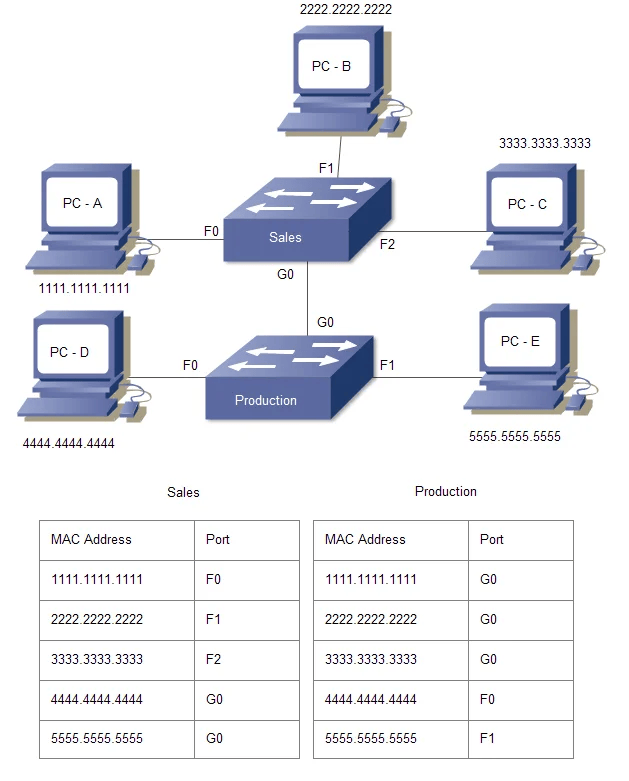
\includegraphics[width=0.8\textwidth]{imgs/tabelamac.png}
\legend{Fonte: \citeonline{CNN2026Lamix}, convertida para png pelo Autor}
\end{figure}

Esta tabela MAC é construída pelo próprio switch, por meio do processo de aprendizado de endereços: a cada frame recebido em uma porta, o switch registra o endereço MAC de origem e o associa a essa porta, montando a tabela de forma dinâmica conforme o tráfego passa pelo equipamento.

\subsection{Camada 3: Camada de Rede}
A camada de Rede \cite{wikipedia2024rede} define o caminho dos dados por meio dos algorítmos de roteamento, como o RIP, que conta o número saltos como métrica de eficácia (mas não leva em conta o tempo de atraso possível em cada salto), ou o OSPF (Open Shortest Path First), que tem como base o algorítmo de Dijkstra; é nessa camada que operam os switches de camada 3, que comunicam sub-redes.

Ela utiliza os protocolos IP e ICMP.
IP \cite{wikipedia2026ip}: Envia datagramas sem garantias, podendo chegar em parte desordenados, duplicados ou mesmo faltantes.
ICMP \cite{wikipedia2026icmp}: Composto principalmente de Echo Request e Echo Reply, ele é utilizado quando se quer verificar uma falha de comunicação entre dois dispositivos, com o comando PING.

Na camada de Rede também são definidos o IP e as subredes, por meio do mascaramento de IP, para conferir mais organizadas e seguras, isolando máquinas em subredes separadas.
\section{Qual a diferença entre adotar uma solução proprietária como o sistema operacional Windows quando comparado a adoção de uma solução Open source como o sistema operacional Ubuntu? Quais seriam os pontos negativos e positivos de cada abordagem?}

Uma das principais diferenças entre as duas abordagens e uma das primeiras a ser destacadas é o custo. Sistemas proprietários como o Windows exigem aquisição de licença via pagamento, enquanto sistemas Open Source como o Ubuntu podem ser simplesmente baixados gratuitamente. Todavia essa diferença não se resume simplesmente ao preço de aquisição. Uma vez que em geral as pessoas estão mais acostumadas com soluções proprietárias, a adoção de soluções gratuitas também podem gerar custos indiretos, como treinamento de equipe e eventual contratação de suporte especializado, de modo que o custo total de adoção nem sempre acompanha o custo da licença, especialmente para empresas grandes que não são da área de tecnologia (áreas com mais profissionais não familiarizados com soluções Open-Source que e requerem mais treino e adaptação).

Ademais, soluções proprietárias como o Windows não oferecem transparência quanto aos seus mecanismos internos, devido a sua natureza fechada, o que impede a auditoria pública do código e mantém pontos de falha desconhecidos sob segurança por obscuridade, prática já considerada ultrapassada. Já códigos Open Source como o Ubuntu, tem o código-fonte amplamente auditável pela comunidade, permitindo maior conhecimento sobre os processos em execução e de forma geral reduzindo a presença de bloatware. Essa abertura de código também garante flexibilidade, uma vez que o usuário ou a empresa que adota Open Source pode modificar o sistema livremente para adequá-lo às próprias necessidades, algo que soluções proprietárias como o Windows não permitem.

Notar-se-á que ao contrário do que se é comumente pensado, a natureza de Open Source não significa a completa ausência de Bloatware ou telemetria. Destaca-se que há, por exemplo, a coleta de telemetria no Ubuntu, nominalmente os pacotes "Popularity Contest"~\cite{popularityContest} (desabilitado por padrão) e o "Ubuntu Report"~\cite{ubuntuReport} (que na época era opt-out, vindo selecionado na instalação por padrão, hoje foi substituido pelo "Ubuntu Insights"~\cite{ubuntuInsights}, que por sua vez é opt-in). Todavia, a coleta de telemetria em soluções Open Source é geralmente mais transparente, com a possibilidade de auditoria do código-fonte e geralmente opt-in ou ao menos com opção de desativação, enquanto soluções proprietárias como o Windows não permitem tal auditoria e podem estar ocultas ao usuário.

Outro ponto relevante é a dependência de fornecedor. A adoção do Windows tende a atrelar a empresa a todo um ecossistema Microsoft (Active Directory, Office, .NET, entre outros), criando um ciclo vicioso no qual as únicas soluções disponíveis são as do fornecedor e/ou parceiros. Soluções Open Source, por seu direito de fork, reduzem essa dependência, embora as múltiplas distribuições possam gerar fragmentação e exigir mais cuidado na escolha da distro adequada e confusão sobre qual fork exotérica obscura usar.

Outra diferença está em quem responde pelo funcionamento do sistema. Ao licenciar o Windows, a empresa contrata um fornecedor identificável, de quem pode exigir prazo de resposta e correção, em contrapartida, as licenças Open Source fornecem o software no estado em que se encontra, e excluem garantia. Deixando assim o risco com quem adota a ferramenta, salvo em casos de contratação de suporte comercial como o Ubuntu Pro. Isso significa que empresas podem contratar um SLA diretamente com a Microsoft, o que não seria possível (ao menos não no mesmo nível) em soluções Open Source.

\subsection{Comparação em ambientes de servidor}
% TODO: Re-ver esse parágrafo
A vantagem de compatibilidade destacada para o Windows é inerente à sua versão de desktop e se inverte no ambiente de servidores, onde o Linux predomina~\cite{linuxPreferedServer}. Desde 2017, a totalidade dos quinhentos supercomputadores mais rápidos do mundo executa Linux~\cite{top500Computers}, e a própria Microsoft em 2019 informou que maior parte das máquinas virtuais hospedadas no Azure já utilizava o sistema~\cite{azureUsesLinux}. Concorrem para esse quadro o licenciamento por núcleo, que penaliza o crescimento horizontal do parque, o menor consumo de recursos de uma instalação sem interface gráfica, a administração remota por linha de comando e o fato de o software de servidor ser majoritariamente desenvolvido tendo o Linux como alvo primário.

O Windows Server 2025 é licenciado por núcleo físico, com mínimo de oito núcleos por processador e dezesseis por servidor, vendidos em pacotes, sendo US\$ 1.176 pelo pacote de dezesseis núcleos da edição Standard e US\$ 6.771 pela Datacenter~\cite{windowsServerPricing}. Sobre isso ainda incidem as CALs, licenças de acesso exigidas de cada usuário ou dispositivo que autentica no domínio e usa compartilhamento de arquivos~\cite{windowsServerPricing}, e o acesso remoto por RDS cobra uma CAL própria. Este último é de particular destaque, pois significa que o custo cresce também com o número de pessoas na empresa acessando o servidor por RDS, independentemente dos custos do servidor em si.

Outro ponto significativo na operação de um servidor é o reinício para aplicar updates. Atualização do Windows Server requerem reboot para aplicação de mudanças, o que significa uma manutenção programada em serviços sem redundancia ou a redução da capacidade máxima. O Windows Server 2025 trouxe o hotpatching, que aplica a maior parte das correções com a máquina em execução, e mesmo assim mantém cerca de quatro reinícios por ano para as atualizações de baseline~\cite{hotpatchMicrosoft, hotpatchAnuncio}. O recurso exige edição Standard ou Datacenter conectada ao Azure Arc e foi lançado em julho de 2025 cobrando US\$ 1,50 por núcleo de CPU ao mês inicialmente~\cite{hotpatchMicrosoft, hotpatchAnuncio}. A Microsoft ouviu as críticas da comunidade e zerou a cobrança em 15 de maio de 2026~\cite{hotpatchGratuito}, mas manteve a exigência do Azure Arc.

No Ubuntu o equivalente é o Livepatch, que corrige o kernel em execução e vem incluso no Ubuntu Pro, gratuito em até cinco máquinas de uso pessoal e US\$ 500 por ano por servidor no plano pago~\cite{ubuntuProPricing}. Este Livepatch, porém, não cobre todas as atualizações, somente as vulnerabilidades de kernel classificadas como alta ou crítica, e não envolve as atualizações em glibc, OpenSSL, systemd ou microcódigo, que continuam exigindo atualização de pacote e reinício~\cite{livepatchEscopo}. Todavia, isso significa que a máquina reinicia no momento que a equipe escolher, não quando o CVE for publicado.

Todavia, no caso do Windows, é importante destacar sua funcionalidade de controlador de domínio, o Active Directory~\cite{activeDirectory} e o Group Policy~\cite{groupPolicy} não possuem uma ferramenta com maturidade comparavel no ecossistema aberto. Esta função é de extrema importância para escritórios corporativos rodando múltiplos desktops, e é um ponto de destaque do Windows.


\subsection{Pontos Positivos e Negativos:}
\subsubsection{Windows:}
Positivos:
\begin{itemize}
	\item Por ser o SO mais utilizado, é compatível com quase todos os aplicativos desktop utilizados no mundo, desde ferramentas profissionais até jogos;
	\item Suporte profissional direto do fabricante, incluindo suporte 24 horas em planos corporativos;
	\item Facilidade de uso: o design e layout do Windows é aquele ao qual a maioria dos profissionais está acostumada, funcionando como padrão de UI usabilidade;
	\item Active Directory e Group Policy para ambientes corporativos;
	\item Melhor suporte a drivers e hardware, pois fabricantes costumam priorizar compatibilidade com Windows.
\end{itemize}

Negativos:
\begin{itemize}
	\item Custo da licença;
	\item Segurança por obscuridade;
	\item Bloatware;
	\item Obsolescência de hardware imposta por novas versões;
	\item Falta de transparência;
	\item Vulnerabilidades mais conhecidas e exploradas, por ser o SO mais utilizado;
	\item Atualizações forçadas e coleta de telemetria, com pouco controle do usuário sobre esses processos;
	\item Ciclo vicioso de compatibilidade em torno do ecossistema Microsoft.
\end{itemize}

\subsubsection{Ubuntu:}
Positivos:
\begin{itemize}
	\item Não há custo de licença;
	\item Transparência e código auditável pela comunidade;
	\item Comunidade colaborativa, que troca constantemente informações, dados e guias;
	\item Maior segurança em partes, pois a ausência de segurança por obscuridade favorece a descoberta e correção de falhas pela própria comunidade, muito embora nem sempre isso ocorra (vide mais detalhes na Q3);
	\item Flexibilidade para modificar o código-fonte e adequar o sistema à realidade de cada usuário ou empresa;
	\item Redução da dependência de uma única empresa fornecedora;
	\item Suporte LTS longo e menor exigência de hardware;
	\item Disponibilidade de suporte profissional pago para empresas que precisam de SLA formal, como o Ubuntu Pro da Canonical, o que reduz a distância em relação ao suporte oferecido por soluções proprietárias, embora em uma escala menor se comparado à Microsoft.
\end{itemize}

Negativos:
\begin{itemize}
	\item Menor compatibilidade com aplicativos de desktop, por ter parcela do mercado consumidor muito menor que do Windows;
	\item Suporte a hardware e drivers mais limitado, sobretudo para periféricos e componentes recentes;
	\item Falhas de segurança conhecidas publicamente enquanto ainda estão sendo corrigidas\footnote{Embora a descoberta destas vulnerabilidades possa ser oculta durante o processo de reparo, o código vulnerável em si é público. Isso permite a descoberta do erro, assim como é possível chamar a atenção a essas falhas por meio dos commits de correção. Estas publicações permitem a chamada n-day vulnerability, na qual se aproveita o tempo entre o patch e os usuários efetivamente aplicarem as atualizações para realizar o exploit de uma falha, esta janela é geralmente considerada entre 60 e 150 dias~\cite{nDay}} além de outras formas de patch gap~\cite{patchGap};
	\item Fragmentação entre distribuições, o que pode dificultar a escolha e a padronização dentro de uma organização;
	\item Necessidade de treinamento da equipe, caso não haja familiaridade com o sistema.
\end{itemize}

Por tais razões, na utilização de desktops corporativos o Windows continua sendo a escolha principal, pela compatibilidade de aplicativos e drivers e pela usabilidade. Para servidores e infraestrutura o argumento se inverte, e a escolha é o Ubuntu Server por motivos de preço, compatibilidade, e eficiência.
\section{Q3. O que seria um projeto Open source? Como empresas podem adotar tais tecnologias e o que isso acarreta?}

Um projeto Open Source é aquele feito colaborativamente por voluntários (ou incomumente, por profissionais pagos) e com o código fonte não compilado disponível para o público geral (por isso o nome código aberto), normalmente por sites como Github. Isso permite que quaisquer pessoas ofereçam sugestões de mudanças, que podem ou não ser acatadas e anexadas ao projeto principal. Projetos Open Source não precisam de pagamento de licença para serem utilizados, podendo ser instalados, distribuídos e modificados livremente.
Empresas podem adotar estas tecnologias simplesmente as baixando e utilizando (juntamente com um treinamento adequado). Ademais, uma vez que projetos open Source podem ser modificados livremente, é plenamente adequado que uma empresa modifique o código para que o programa melhor se adeque à realidade da companhia.

\bibliography{referencias}


\end{document}
